\documentclass{article}
\usepackage[utf8x]{inputenc}
\usepackage{ucs}
\usepackage{amsmath} 
\usepackage{amsfonts}
\usepackage{upgreek}
\usepackage[english,russian]{babel}
\usepackage{graphicx}
\usepackage{float}
\usepackage{textcomp}
\usepackage{hyperref}
\usepackage{geometry}
  \geometry{left=2cm}
  \geometry{right=1.5cm}
  \geometry{top=1.5cm}
  \geometry{bottom=2cm}
\usepackage{tikz}
\usepackage{ccaption}
\usepackage{multicol}

\usepackage{listings}
%\setlength{\columnsep}{1.5cm}
%\setlength{\columnseprule}{0.2pt}


\begin{document}
\pagenumbering{gobble}

\lstset{
  language=C++,
  basicstyle=\linespread{1.1}\ttfamily,
  columns=fixed,
  fontadjust=true,
  basewidth=0.5em,
  keywordstyle=\color{blue}\bfseries,
  commentstyle=\color{gray},
  stringstyle=\ttfamily\color{orange!50!black},
  showstringspaces=false,
  %numbers=false,
  numbersep=5pt,
  numberstyle=\tiny\color{black},
  numberfirstline=true,
  stepnumber=1,      
  numbersep=10pt,
  backgroundcolor=\color{white},
  showstringspaces=false,
  captionpos=b,
  breaklines=true
  breakatwhitespace=true,
  xleftmargin=.2in,
  extendedchars=\true,
  keepspaces = true,
  tabsize=4,
}
\lstset{ literate={~}{{\raisebox{0.5ex}{\texttildelow}}}{1} }

\title{Семинар \#8: Умные указатели и классы представления \vspace{-5ex}}\date{}\maketitle

\section*{Проблема ошибок при работе с динамической памятью}
Одни из частых ошибок, которые возникают при программировании на языке C и C++, являются утечки памяти. Утечка памяти возникает тогда, когда была выделена память в куче с помощью функции \texttt{malloc}, но эта память не была освобождена с помощью функции \texttt{free}. Аналогичная проблема возникает и при использовании операторов \texttt{new} и \texttt{delete}:
\begin{lstlisting}
void func(int n) 
{
    int* p = new int[n];
    // забыли сделать delete[] p;
}

int main() 
{
    func(100); // Утечка
    func(200); // Ещё одна утечка
}
\end{lstlisting}

Например, в этой программе утечка памяти происходит в функции \texttt{func}, так как в ней выделяется память с помощью \texttt{new[]}, но не освобождается с помощью \texttt{delete[]}. После выхода из функции \texttt{func} мы не сможем освободить эту память, даже если бы хотели, так как мы не знаем чему равен указатель \texttt{p}.

Может показаться, что такую ошибку легко увидеть, но на самом деле, это не всегда верно. Программа может быть очень большой, выделений памяти может быть очень много, выделение памяти может происходить в одной функции, а освобождение этой памяти происходить в другой функции и т. д. 
Сложности добавляет использование исключений. Ведь если где-то в функции будет брошено исключение, то произойдёт выход из функции без освобождение выделенной в этой функции памяти. Рассмотрим, например, такую функцию, содержащую утечку памяти:
\begin{lstlisting}
void func(int n) 
{
    int* p = new int[n];
    int* q = new int[n];
	// ...		
    delete[] q;
    delete[] p;
}
\end{lstlisting}
Утечка в данной функции произойдёт, если второй оператор \texttt{new} не сможет выделить память и бросит исключение. Произойдёт выход из этой функции без освобождения памяти на которую указывает указатель \texttt{p}.

Другая проблема, которая может возникнить при ручном выделении памяти, это проблема двойного удаления. Удаление объекта, который уже был удалён, приведёт к неопределённому поведению:
\begin{lstlisting}
int* p = new int[10];
// ...
delete[] p;
// ...
delete[] p; // UB
\end{lstlisting}
Опять же, на таком простом примере эта ошибка очевидна, но в больших программах с большим количеством
использований \texttt{new}/\texttt{delete} памяти такую ошибку может быть трудно заметить.

Хотелось бы иметь способ писать код так, чтобы минимизировать возможные ошибки.



\newpage
\section*{Пишем свой умный указатель}
Давайте используем знания, полученные при изучении C++ и напишем класс, который будет освобождать память за нас. Назовём его \texttt{SmartPointer}, то есть умный указатель. Умный, потому что он сам будет освобождать память. Этот класс должен конструироваться от обычного указателя, который указывает память в куче и освобождать память в деструкторе.
\begin{lstlisting}
#include <iostream>

template <typename T>
class SmartPointer
{
private:
    T* pointer;

public:
    SmartPointer(T* pointer) : pointer(pointer) {}
    T& operator*()  const {return *pointer;}
    T* operator->() const {return pointer;}

    ~SmartPointer() 
    {
        std::cout << "Deleting" << std::endl;
        delete pointer;
    }
};

int main()
{
    SmartPointer<int> p = new int(123);
    std::cout << *p << std::endl;
} 
\end{lstlisting}
В этой программе нет утечки памяти, потому что \texttt{delete} вызовется в деструкторе объекта \texttt{q}. 

Однако, у этой реализации умного указателя есть много проблем. Самая главная проблема заключается в том, что не были прописаны конструктор копирования и оператор присваивания. В результате конструктор копирования и оператор присваивания были созданы автоматически. Такие автоматически созданные методы будут просто копировать внутренний указатель в другой объект умного указателя. Это может привести к сеьёзным ошибкам:
\begin{lstlisting}
int main()
{
	SmartPointer<int> p = new int(123);
	SmartPointer<int> q = p;
	// UB: двойной delete
}
\end{lstlisting}
Умный указатель \texttt{q} скопирует указатель в себя поле \texttt{pointer} указателя \texttt{p}. В результате оба умных указателя будут указывать на одно и то же место. Следовательно, в деструкторах  обоих умных указателей будет вызван \texttt{delete} для одного и того адреса. Получилось двойное освобождение, что является неопределённым поведением.

Вообще, для данной реализации умного указателя мы не можем допустить того, чтобы несколько таких умных указателей указывали на один объект в куче. Ведь, если хотя бы один из этих умных указателей будет уничтожен (например, если мы выйдем из области видимости, где данный умный указатель был создан), то он уничтожит и объект в памяти, который в этот момент может использоваться через другие умные указатели. Это неопределённое поведение. Если же все такие умные указатели уничтожатся разом, то все они будут удалять один и тот же объект в своих деструкторах. Это тоже неопределённое поведение.\\


\newpage
Есть два общепринятых способа избежать такой ситуации:
\begin{enumerate}
\item Сделать так, чтобы на один объект в куче мог указывать максимум только один умный указатель. Этот способ использует умный указатель \texttt{std::unique\_ptr}.
\item Завести счётчик и подсчитывать сколько умных указателей указывает на данный объект в куче. Если один из указателей, указывающий на данный объект, уничтожается то счётчик уменьшается на 1. Объект уничтожается только тогда, когда счётчик достигнет нуля (то есть тогда когда уничтожится последний умный указатель, который указывал на данный объект). Этот способ использует умный указатель \texttt{std::shared\_ptr}.
\end{enumerate}


\section*{Умный указатель \texttt{std::unique\_ptr}}
\texttt{std::unique\_ptr} -- это умный указатель из библиотеки \texttt{memory}, который реализует эксклюзивное владение объектом. Этот умный указатель обладает следующими свойствами:
\begin{itemize}
\item \texttt{unique\_ptr} может конструироваться из обычного указателя на объект в куче. При этом этот конструктор является \texttt{explicit}-конструктором, поэтому конструироваться из обычного указателя можно только с помощью прямой инициализации. Объект в куче уничтожается в деструкторе \texttt{unique\_ptr}.
\item Несколько указателей \texttt{unique\_ptr} не могут указывать на один объект в куче. Это достигается благодаря тому, что эти указатели нельзя копировать, но можно перемещать. При перемещении, \texttt{unique\_ptr}, из которого происходит перемещение, перестаёт указывать на объект и становится нулевым.
\item Указатель \texttt{unique\_ptr} может быть нулевым, то есть не указывать никуда. Нулевой \texttt{unique\_ptr} можно получить, если сконструировать объект с помощью конструктора по умолчанию.
\end{itemize}

\begin{lstlisting}
#include <iostream>
#include <memory>

int main()
{
	std::unique_ptr<int> p(new int(10));
	
	std::unique_ptr<int> q1 = p;             // Ошибка, unique_ptr нельзя копировать
	std::unique_ptr<int> q2 = std::move(p);  // ОК, но теперь p стал нулевым, 
	                                         // только q2 указывает на объект в куче
}
\end{lstlisting}


Процесс перемещения умного указателя \texttt{unique\_ptr} представлен на следующем рисунке:

\begin{center}
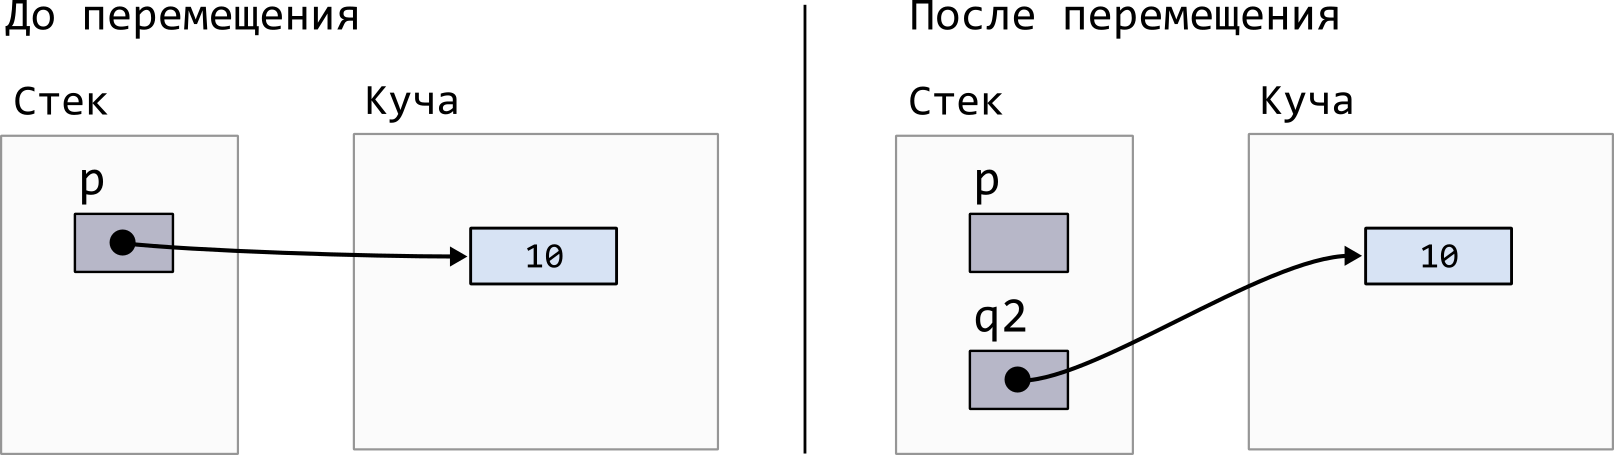
\includegraphics[scale=1]{../images/move_unique_ptr.png}
\end{center}


\newpage
\subsection*{Методы класса \texttt{std::unique\_ptr}}
\begin{itemize}
\item \texttt{operator*} и \texttt{operator->} -- работают аналогично таким же операторам обычного указателя.

\item \texttt{operator bool()} -- оператор приведения к типу \texttt{bool}:
\begin{lstlisting}
std::unique_ptr<int> p(new int(10));
if (p) 
	std::cout << "Yes" << std::endl;
	
std::unique_ptr<int> q;
if (q) 
	std::cout << "No" << std::endl;
\end{lstlisting}


\item \texttt{get} -- возвращает обычный указатель на объект:
\begin{lstlisting}
std::unique_ptr<int> p(new int(10));
int* q = p.get();
\end{lstlisting}

\item \texttt{release} -- после вызова этого метода \texttt{unique\_ptr} перестаёт указывать на объект и становится нулевым. Объект, при этом, не удаляется. Возвращает указатель на объект.
\begin{lstlisting}
std::unique_ptr<int> p(new int(10));
int* q = p.release();
delete q;
\end{lstlisting}

\item \texttt{swap} -- меняет местами значение двух \texttt{unique\_ptr}.
\begin{lstlisting}
std::unique_ptr<int> p(new int(10));
std::unique_ptr<int> q(new int(20));

std::cout << *p << " " << *q << std::endl; 
p.swap(q);
std::cout << *p << " " << *q << std::endl; 
\end{lstlisting}
\end{itemize}

\subsection*{Передача \texttt{std::unique\_ptr} в функции}
Обычно функции принимают \texttt{unique\_ptr} по значению. Умный указатель в такие функции передаётся с использованием семантики перемещения.
\begin{lstlisting}
#include <iostream>
#include <memory>

void func(std::unique_ptr<int> p)
{
	std::cout << *p << std::endl;
}

int main()
{
	std::unique_ptr<int> p(new int(10));
	func(std::move(p));
	
	if (p == nullptr)
		std::cout << "p in main is null" << std::endl;
}
\end{lstlisting}

\newpage
Но можно передавать \texttt{unique\_ptr} и по ссылке. Это менее предпочтительный способ, так как он может быть медленнее. Из-за того, что в функции \texttt{func}, чтобы доступиться до объекта в куче, придётся делать два шага: сначала нужно перейти по ссылке к указателю \texttt{unique\_ptr}, а потом по указателю к объекту в куче.
\begin{lstlisting}
#include <iostream>
#include <memory>

void func(std::unique_ptr<int>& p)
{
	std::cout << *p << std::endl;
}

int main()
{
	std::unique_ptr<int> p(new int(10));
	func(p);
	
	if (p == nullptr)
		std::cout << "p in main is null" << std::endl;
	else
		std::cout << "p = " << *p << std::endl;
}
\end{lstlisting}

\subsection*{Примеры ошибочного использования \texttt{unique\_ptr}}
Нужно понимать, что если \texttt{unique\_ptr} конструируется от обычного указателя, то это должен быть указатель, который пришел из оператора \texttt{new} и никакой другой. В частности нельзя делать следующее:
\begin{itemize}
\item Конструироваться от адреса локальной переменной:
\begin{lstlisting}
int a = 10;
std::unique_ptr<int> p(&a);  // Ошибка
\end{lstlisting}
В этом случае, в деструктроре \texttt{unique\_ptr} будет вызыван \texttt{delete} с адресом локальной переменной. Это конечно приведёт к неопределённому поведению.

\item Конструироваться от адреса полученного из оператора \texttt{new[]}:
\begin{lstlisting}
std::unique_ptr<int> p(new int[100]);  // Ошибка
\end{lstlisting}
В этом случае, в деструктроре \texttt{unique\_ptr} будет вызыван \texttt{delete}, а не нужный нам оператор \texttt{delete[]}. Это также приведёт к UB.
\end{itemize}
Еще одна ошибка может возникнуть, если создать два умных указателя от одного обычного указателя.
\begin{lstlisting}
int* raw = new int(10);
std::unique_ptr<int> p(raw);
std::unique_ptr<int> q(raw);
\end{lstlisting}
В этом случае один умный указатель создаётся независимо от другого и не может проверить, есть ли ещё один указатель, указывающий на тот же объект. Поэтому оба указателя \texttt{p} и \texttt{q} будут указывать на один и тот же объект в куче. Естественно, когда эти указатели уничтожатся, они будут уничтожать объект, на который они указывают и произойдёт двойное удаление одного объекта. Это UB.


\newpage
\subsection*{Функция \texttt{std::make\_unique}}
Чтобы исключить возможность возникновения ошибочных ситуаций, перечисленных выше, для создания умных указателей \texttt{unique\_ptr} следует использовать специальную функцию \texttt{make\_unique}. Эта функция сама, внутри себя, создаёт объект в куче с помощью оператора \texttt{new}, создаёт указатель \texttt{unique\_ptr} на этот объект и возвращает его. Использовать её нужно так:
\begin{lstlisting}
std::unique_ptr<int> p = std::make_unique<int>(10);
\end{lstlisting}
Или ещё лучше так:
\begin{lstlisting}
auto p = std::make_unique<int>(10);
\end{lstlisting}
Интересной особеностью функции \texttt{std::make\_unique} является то, что она принимает на вход не уже сконструированный объект, а \textit{аргументы его конструктора}. Это можно увидеть на следующем примере:
\begin{lstlisting}
#include <iostream>
#include <string>
#include <memory>

class Book
{
private:
	std::string title {};
	int pages         {};
	float price       {};

public:
	Book(const std::string& title, int pages, float price)
		: title(title), pages(pages), price(price)
	{
		std::cout << "Constructor" << std::endl;
	}
	
	Book(const Book& b)
		: title(b.title), pages(b.pages), price(b.price)
	{
		std::cout << "Copy Constructor" << std::endl;
	}
};

int main()
{
	// Правильное использование
	auto p = std::make_unique<Book>("Harry Potter", 100, 200);
	
	// Неравильное использование
	// Будет вызван на один конструктор больше
	auto q = std::make_unique<Book>(Book("Harry Potter", 100, 200));
}
\end{lstlisting}
Это происходит потому что функция \texttt{make\_unique} принимает аргументы по ссылке и конструирует объект внутри себя. Во втором же случае объект \texttt{Book} был создан до входа в функцию \texttt{make\_unique} и в функции был создан заново через конструктор копирования. 

Также заметьте, что \texttt{make\_unique} принимает произвольное количество аргументов произвольных (возможно различных) типов и произвольных(возможно различных) категорий. 



\newpage
\section*{Умный указатель \texttt{std::shared\_ptr}}
\texttt{std::shared\_ptr} -- это умный указатель из библиотеки \texttt{memory}, который реализует паттерн общего владения объектом. Этот умный указатель обладает следующими свойствами:

\begin{itemize}
\item \texttt{shared\_ptr} может конструироваться из обычного указателя на объект в куче. При этом этот конструктор является \texttt{explicit}-конструктором, поэтому конструироваться из обычного указателя можно только с помощью прямой инициализации. \texttt{shared\_ptr} сам корректно уничтожит объект в куче.

\item Несколько указателей \texttt{shared\_ptr} могут указывать на один объект в куче. Объект уничтожится только тогда, когда уничтожится последний \texttt{shared\_ptr}, указывающий на этот объект.

\item Указатель \texttt{shared\_ptr} можно копировать и присваивать. При копировании создастся новый указатель \texttt{shared\_ptr}, который будет указывать на тот же объект.

\item Указатель \texttt{shared\_ptr} можно перемещать. При перемещении, \texttt{shared\_ptr}, из которого происходит перемещение, станет пустым.

\item Указатель \texttt{shared\_ptr} может быть нулевым, то есть никуда не указывать. Нулевой \texttt{shared\_ptr} можно получить, если сконструировать объект с помощью конструктора по умолчанию.
\end{itemize}

\begin{lstlisting}
#include <iostream>
#include <memory>

int main()
{
	std::shared_ptr<int> p(new int(10));
	
	std::shared_ptr<int> q1 = p;             // ОК, теперь 2 указателя указывают на объект
	std::shared_ptr<int> q2 = std::move(p);  // ОК, но теперь p стал нулевым, 
	                                         // q1 и q2 указывает на один объект в куче
}
\end{lstlisting}
\quad\\

Разберём этот участок кода по шагам, при этом будем смотреть, что происходит в памяти. Внутри объекта \texttt{shared\_ptr} хранится указатель на объект в куче, а также указатель на счётчик ссылок.
\quad\\
\quad\\

\begin{minipage}{0.45\textwidth}
\begin{lstlisting}
// Создаём новый указателя shared_ptr
std::shared_ptr<int> p(new int(10));
\end{lstlisting}
\end{minipage}
\begin{minipage}{0.5\textwidth}
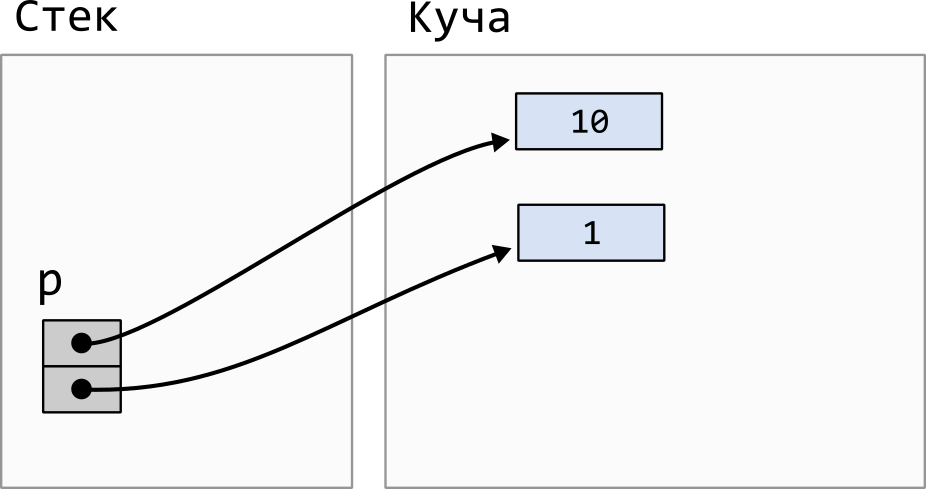
\includegraphics[scale=1]{../images/shared_ptr1.png}
\end{minipage}
\quad\\
\quad\\

\begin{minipage}{0.45\textwidth}
\begin{lstlisting}
// Создаём копию указателя
std::shared_ptr<int> q1 = p;
\end{lstlisting}
\end{minipage}
\begin{minipage}{0.5\textwidth}
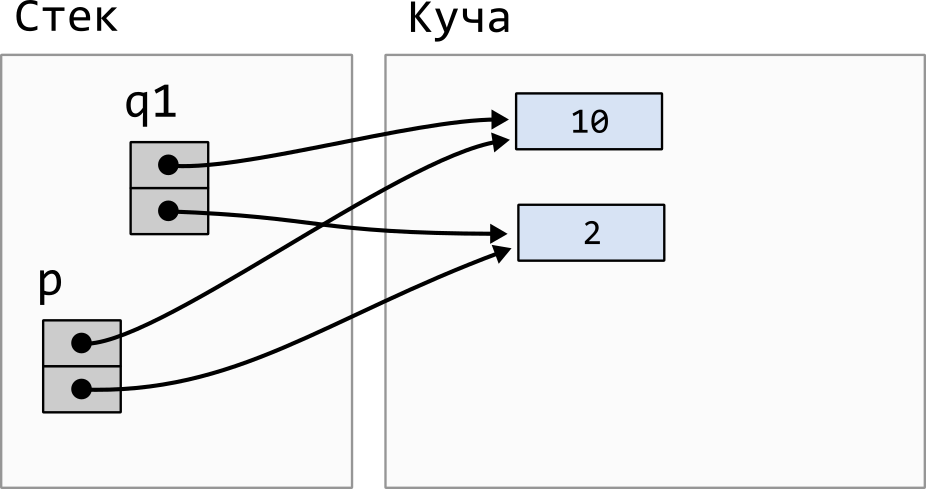
\includegraphics[scale=1]{../images/shared_ptr2.png}
\end{minipage}
\quad\\
\quad\\

\begin{minipage}{0.45\textwidth}
\begin{lstlisting}
// Перемещаем указатель p в q2
std::shared_ptr<int> q2 = std::move(p);
\end{lstlisting}
\end{minipage}
\begin{minipage}{0.5\textwidth}
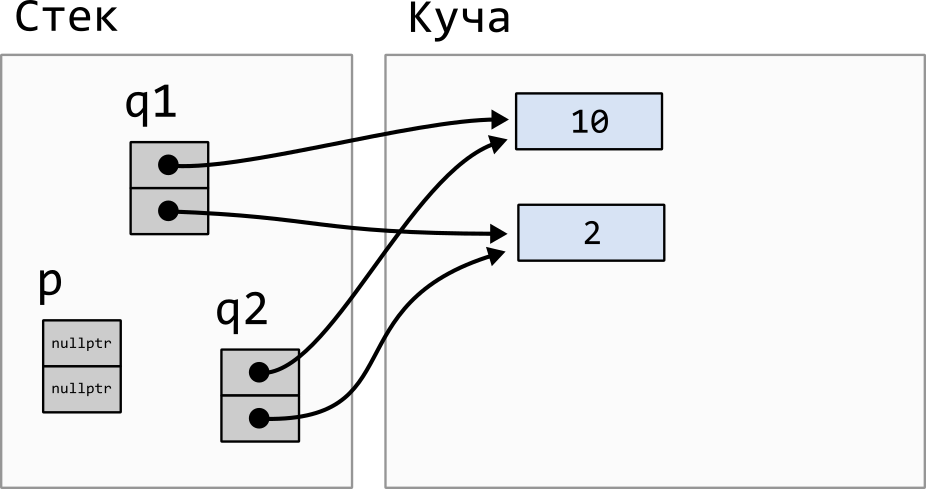
\includegraphics[scale=1]{../images/shared_ptr3.png}
\end{minipage}



\subsection*{Методы класса \texttt{shared\_ptr}}
\begin{itemize}
\item \texttt{operator*} и \texttt{operator->} -- работают аналогично таким же операторам обычного указателя.

\item \texttt{operator bool()} -- оператор приведения к типу \texttt{bool}:
\begin{lstlisting}
std::shared_ptr<int> p(new int(10));
if (p) 
	std::cout << "Yes" << std::endl;
	
std::shared_ptr<int> q;
if (q) 
	std::cout << "No" << std::endl;
\end{lstlisting}


\item \texttt{get} -- возвращает обычный указатель на объект:
\begin{lstlisting}
std::shared_ptr<int> p(new int(10));
int* q = p.get();
\end{lstlisting}


\end{itemize}

\newpage
\subsection*{Передача класса \texttt{shared\_ptr} в функции}

\subsection*{Примеры ошибочного использования \texttt{shared\_ptr}}

\subsection*{Функция \texttt{std::make\_shared}}


\section*{Циклические ссылки}

\newpage
\section*{Указатель \texttt{std::weak\_ptr}}

\section*{Пользовательский удалитель (\textit{custom deleter}) для умных указателей}

\section*{Класс представления \texttt{std::string\_view}}

\section*{Класс представления \texttt{std::span}}



\end{document}